\documentclass[11pt,a4paper]{article}

\usepackage[margin=1in]{geometry}
\usepackage{titlesec}
\usepackage{enumitem}
\usepackage{hyperref}
\usepackage{parskip}
\usepackage{graphicx}
\usepackage{float}
\usepackage{booktabs}
\usepackage{amsmath}
\usepackage{amssymb}

\hypersetup{colorlinks=true, linkcolor=blue, urlcolor=blue}

\titleformat{\section}{\large\bfseries}{\thesection}{0.5em}{}
\titleformat{\subsection}{\normalsize\bfseries}{\thesubsection}{0.5em}{}
\setlist{leftmargin=1.4em, topsep=2pt, itemsep=2pt}

\title{\vspace{-1.5cm}\textbf{PKCERT AI \& Software Development Internship \\ Task 26: Introduction to Transformers \& the Attention Mechanism (Conceptual)}}
\author{Abdullah Amir}
\date{AI and Software Development \\ 11 August 2026}

\begin{document}

\maketitle
\vspace{-0.8cm}

Full code lives in \texttt{Day\_26.ipynb} and the standalone scripts it is built from.
\textbf{This task is explicitly conceptual}, per the brief: no attention mechanism or
Transformer block is implemented from scratch as a trainable component. Parts A/B are
mathematical derivations, illustrated with small NumPy worked examples and visualizations
(exactly what the brief itself requests -- a toy attention calculation, a plotted positional
encoding matrix, architecture diagrams) rather than a production implementation. Only Part C
requires code, and it uses an existing pretrained model (DistilBERT, via Hugging Face
\texttt{transformers}) as-is. \textbf{PyTorch 2.13.0 (CPU-only build)}, random seed
\textbf{42} throughout.

% ----------------------------------------------------------------
\section*{Part A: From Recurrence to Attention}

\textbf{A1 -- structural bottlenecks of recurrence (referencing Task 25).} Three bottlenecks,
measured not just asserted in Task 25: (1) \emph{sequential computation} -- $h_t=f(x_t,h_{t-1})$
forces strictly sequential processing, no parallelism across time; (2) \emph{long-range
dependency decay} -- Task 25's own vanishing-gradient demo measured a Jacobian-product norm
collapsing to $\sim1.17\times10^{-18}$ after 60 BPTT steps at spectral radius 0.5, and the
LSTM's cell-state highway mitigates but does not eliminate this; (3) \emph{fixed-size context
propagation} -- the entire history is compressed into one fixed-dimensionality $h_t$ (or
$(h_t,c_t)$) regardless of sequence length. Attention targets all three: O(1)-length paths
between any two positions, no fixed-size bottleneck (every position's own representation
stays available), and no sequential-computation constraint.

\textbf{A2 -- Bahdanau/Luong attention.} An encoder produces hidden states $h_1,\ldots,h_{T_x}$;
a decoder state $s_{t-1}$ computes an \textbf{alignment score} against each: Bahdanau
(additive) $e_{t,i}=v^\top\tanh(W_a s_{t-1}+U_a h_i)$, Luong (multiplicative)
$e_{t,i}=s_t^\top h_i$ (dot) or $s_t^\top W_a h_i$ (general). Scores are normalized into
\textbf{attention weights} $\alpha_{t,i}=\exp(e_{t,i})/\sum_j\exp(e_{t,j})$, defining the
\textbf{context vector} $c_t=\sum_i \alpha_{t,i}h_i$ -- direct access to the entire encoder
sequence at every decoder step, generalized by scaled dot-product attention below.

\textbf{A3 -- scaled dot-product attention, derived.}
$$\text{Attention}(Q,K,V) = \text{softmax}\left(\frac{QK^\top}{\sqrt{d_k}}\right)V$$
$Q\in\mathbb{R}^{n_q\times d_k}$ (queries), $K\in\mathbb{R}^{n_k\times d_k}$ (keys),
$V\in\mathbb{R}^{n_k\times d_v}$ (values). $QK^\top$ is a batched matrix-multiply version of
every A2 alignment score computed at once; softmax-normalizing rows and multiplying by $V$
generalizes A2's $\alpha_{t,i}$ and $c_t$.

\textbf{Why $1/\sqrt{d_k}$ is necessary.} For $q,k$ with i.i.d.\ zero-mean, unit-variance
entries, $\text{Var}(q\cdot k) = \sum_{i=1}^{d_k}\text{Var}(q_ik_i) = d_k$ -- unscaled dot
products' standard deviation grows as $\sqrt{d_k}$, easily reaching magnitudes of $\pm20$ for
typical $d_k$ (e.g.\ 64). Softmax's gradient
$\partial\text{softmax}(x)_i/\partial x_j = \text{softmax}(x)_i(\delta_{ij}-\text{softmax}(x)_j)$
vanishes as its output saturates toward one-hot, exactly what large-magnitude inputs cause.
Dividing by $\sqrt{d_k}$ rescales $q\cdot k$ back to unit variance \emph{independent of
$d_k$}, keeping softmax well-conditioned -- the same saturating-nonlinearity-plus-large-
preactivation gradient-vanishing mechanism Task 25 analyzed for tanh/sigmoid, occurring
inside softmax instead.

\textbf{A4 -- worked numerical example.} 4 toy tokens (river, flows, bank, money),
$d_k{=}d_v{=}3$, hand-chosen so ``bank'' is ambiguous between geography and finance.

\begin{figure}[H]
    \centering
    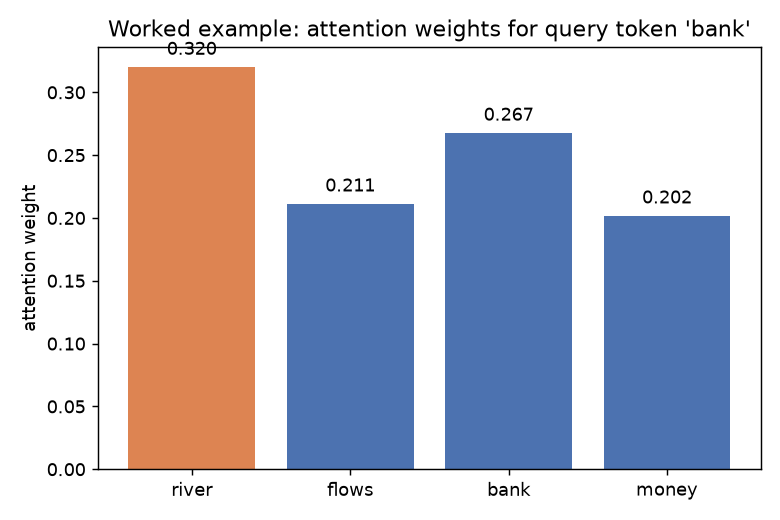
\includegraphics[width=0.55\textwidth]{figures/part_a_worked_example.png}
    \caption{Worked example: attention weights for query token ``bank''.}
\end{figure}

\begin{table}[H]
\centering
\begin{tabular}{lrrr}
\toprule
\textbf{Key/value} & \textbf{Raw score} & \textbf{Scaled score} & \textbf{Attention weight} \\
\midrule
river & +0.900 & +0.520 & \textbf{0.3199} \\
flows & +0.180 & +0.104 & 0.2111 \\
bank  & +0.590 & +0.341 & 0.2675 \\
money & +0.100 & +0.058 & 0.2016 \\
\bottomrule
\end{tabular}
\end{table}

The query for ``bank'' attends most strongly to ``river'' (weight 0.320), pulling
geography-flavored information into bank's contextualized representation -- the toy
mechanism behind attention-based word-sense disambiguation.

% ----------------------------------------------------------------
\section*{Part B: Transformer Architecture}

\textbf{B1 -- multi-head attention.} A single attention computation produces one weighted
average per query -- if two tokens are relevant for different reasons (syntax vs.\
coreference), one head must blend both. With $h$ heads ($d_k{=}d_v{=}d_{\text{model}}/h$):
$\text{head}_i = \text{Attention}(QW_i^Q, KW_i^K, VW_i^V)$,
$\text{MultiHead}(Q,K,V)=\text{Concat}(\text{head}_1,\ldots,\text{head}_h)W^O$. Empirically
(Clark et al.\ 2019), different heads specialize: local/positional, syntactic-dependency,
coreference-like, or broad/global patterns -- emergent from training, not hand-designed.

\textbf{B2 -- positional encoding.} Self-attention is permutation-\emph{equivariant}, with no
term depending on position $t$ -- unlike the RNN's order-dependent-by-construction recurrence.
Sinusoidal PE:
$$PE(pos,2i)=\sin(pos/10000^{2i/d_{\text{model}}}), \quad PE(pos,2i{+}1)=\cos(pos/10000^{2i/d_{\text{model}}})$$

\begin{figure}[H]
    \centering
    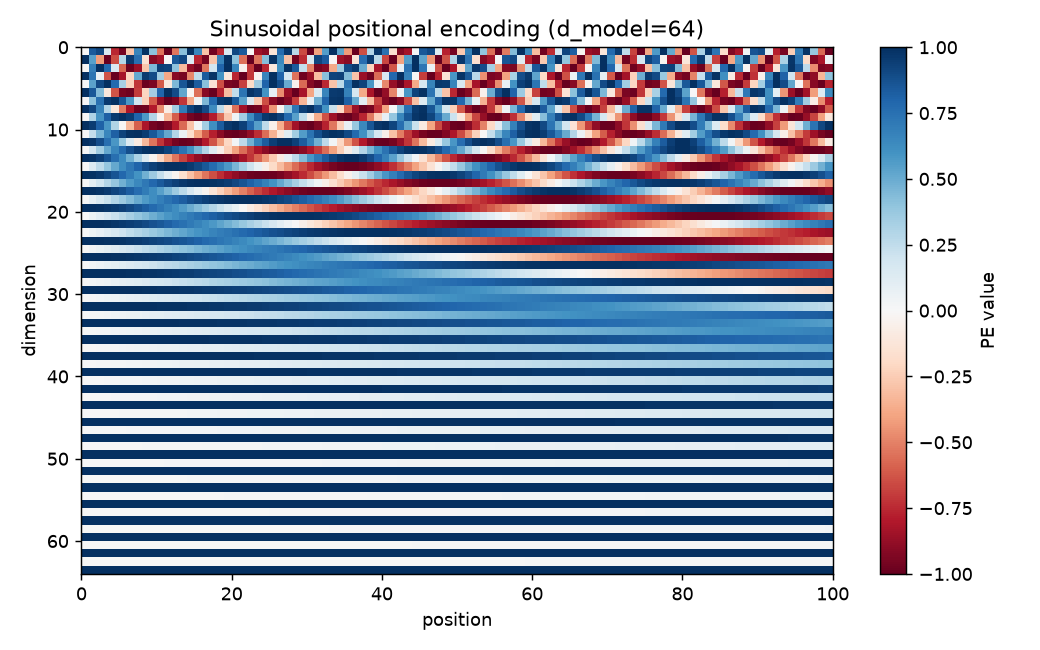
\includegraphics[width=0.75\textwidth]{figures/part_b_positional_encoding.png}
    \caption{Sinusoidal positional encoding, $d_{\text{model}}=64$.}
\end{figure}

Varying frequency per dimension pair gives each position a unique multi-resolution
fingerprint. \textbf{Relative-position representability}: via
$\sin(a{+}b)=\sin a\cos b+\cos a\sin b$, $\cos(a{+}b)=\cos a\cos b-\sin a\sin b$, each
frequency's $(\sin,\cos)$ pair is rotated by a fixed $2\times2$ matrix $R(\omega_i k)$
depending only on offset $k$ -- stacking these block-diagonally gives $M_k$ with
$PE(pos{+}k)=M_k\,PE(pos)$ for \emph{every} $pos$, \textbf{numerically confirmed to
$1.11\times10^{-16}$ max abs.\ error}. Contrast learned positional embeddings: no
hand-designed bias, simpler, but a hard-coded max length and no guaranteed relative-position
structure -- many later models (BERT, GPT-2) used learned embeddings anyway once
train/inference length mismatch mattered less in practice.

\textbf{B3 -- encoder/decoder blocks.}

\begin{figure}[H]
    \centering
    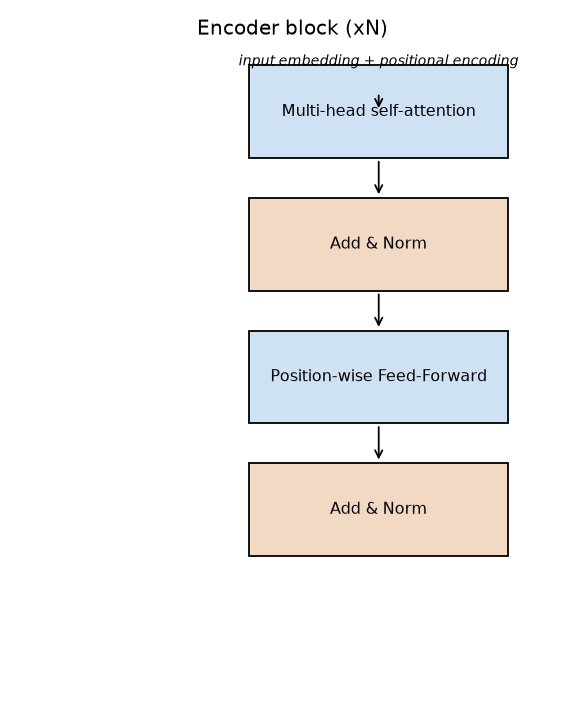
\includegraphics[width=0.42\textwidth]{figures/part_b_encoder_block.png}
    \hfill
    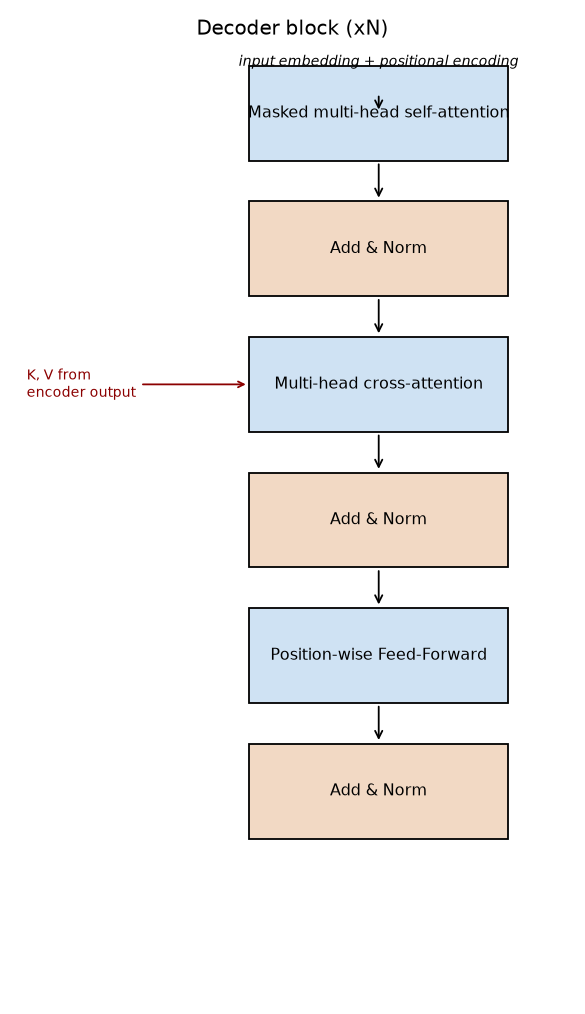
\includegraphics[width=0.42\textwidth]{figures/part_b_decoder_block.png}
    \caption{Encoder block (left) and decoder block (right), each $\times N$.}
\end{figure}

Encoder: multi-head self-attention $\to$ Add\&Norm $\to$ position-wise FFN $\to$ Add\&Norm.
Decoder: masked self-attention $\to$ Add\&Norm $\to$ cross-attention (Q from decoder, K/V from
encoder -- generalizing A2's alignment mechanism) $\to$ Add\&Norm $\to$ FFN $\to$ Add\&Norm.
\textbf{Causal masking}: sets $QK^\top$ entries with $t'>t$ to $-\infty$ before softmax, so
future positions get exactly 0 attention weight -- required because training-time attention
must match what's genuinely available at autoregressive inference time, when future tokens
don't exist yet.

\textbf{B4 -- residual connections and LayerNorm.} $\text{output}=x+\text{Sublayer}(x)$ gives
$dL/dx = dL/d(\text{output})\cdot(1+d(\text{Sublayer}(x))/dx)$ -- an unattenuated
identity-shortcut gradient path regardless of the sublayer's own Jacobian. Structurally
\emph{identical} to the LSTM's cell-state highway (Task 25: $\partial c_t/\partial
c_{t-1}=f_t$), just applied across stacked \emph{layers} instead of \emph{time steps} --
without it, stacking $N$ Transformer layers risks the same vanishing-gradient problem Task 25
derived for deep unrolled RNNs. LayerNorm normalizes each token independently across its
feature dimension (unlike BatchNorm's across-batch normalization), suiting variable-length
sequences and stabilizing deep-stack training.

\textbf{B5 -- complexity.} Self-attention: $O(n^2 d)$ ($QK^\top$ and $(\cdot)V$ are both
$n^2$-scaling matrix products). Recurrence: $O(nd^2)$ ($n$ sequential $d\times d$
matrix-vector products).

\begin{figure}[H]
    \centering
    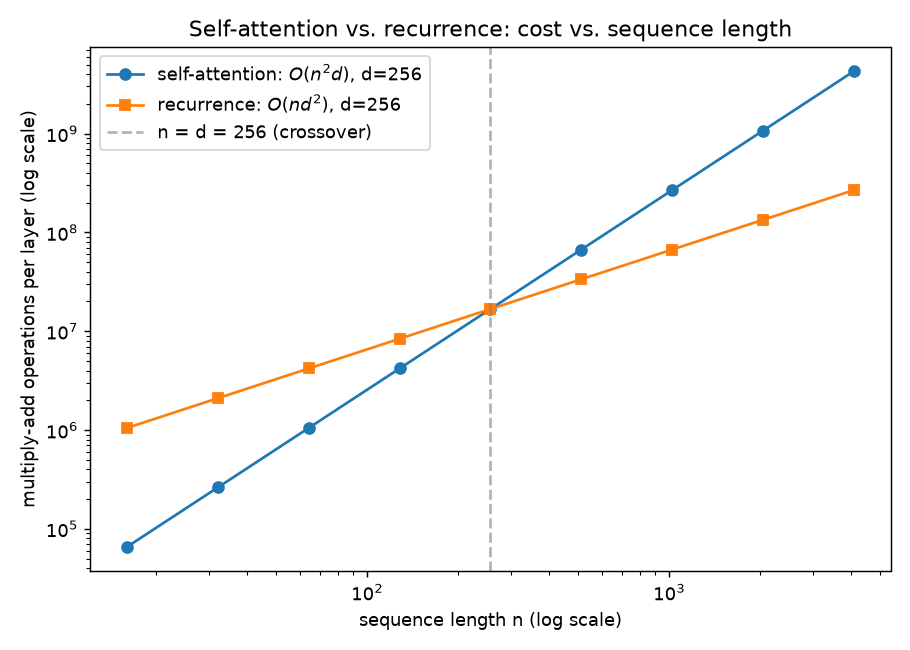
\includegraphics[width=0.7\textwidth]{figures/part_b_complexity.png}
    \caption{Self-attention vs.\ recurrence: cost vs.\ sequence length ($d=256$).}
\end{figure}

For $n<d$ (this task's short AG News sequences), attention is cheaper per layer; for $n>d$
(long documents), attention's $O(n^2)$ memory for the full attention matrix becomes the
binding constraint. \textbf{Documented mitigation}: Longformer's (Beltagy et al.\ 2020)
sliding-window + global-token attention, $O(n\cdot w\cdot d)$ for window $w\ll n$ -- referenced,
not derived.

% ----------------------------------------------------------------
\section*{Part C: Applied Transformer Analysis}

\textbf{C1 -- model selection.} \textbf{DistilBERT} (\texttt{distilbert-base-uncased}), via
Hugging Face \texttt{transformers}: a 6-layer, 768-hidden, 12-head encoder distilled from
BERT-base, 66M params ($\sim$40\% smaller, $\sim$97\% of BERT's GLUE performance per Sanh et
al.\ 2019). Chosen for architecture fit (standard encoder-only Transformer, right family for
classification), compute budget (this CPU-only environment shaped every applied task in this
internship), and library-provided classification head requiring no architectural
modification.

\textbf{C2 -- pipeline.} \textbf{WordPiece} tokenization (BERT's native subword scheme --
unseen words decompose into known subword pieces rather than a single \texttt{<unk>}, unlike
Task 25's from-scratch word-level tokenizer). Input format:
\texttt{[CLS] tok\_1...tok\_n [SEP]}, padded/truncated to 64 tokens with an attention mask.
Classification head: the library's own pooled-\texttt{[CLS]} $\to$ pre-classifier linear+ReLU
$\to$ dropout $\to$ linear-to-4-classes stack.

\textbf{C3 -- attention visualization.} Layer 4, head 4, on a sample Mars-rover article.

\begin{figure}[H]
    \centering
    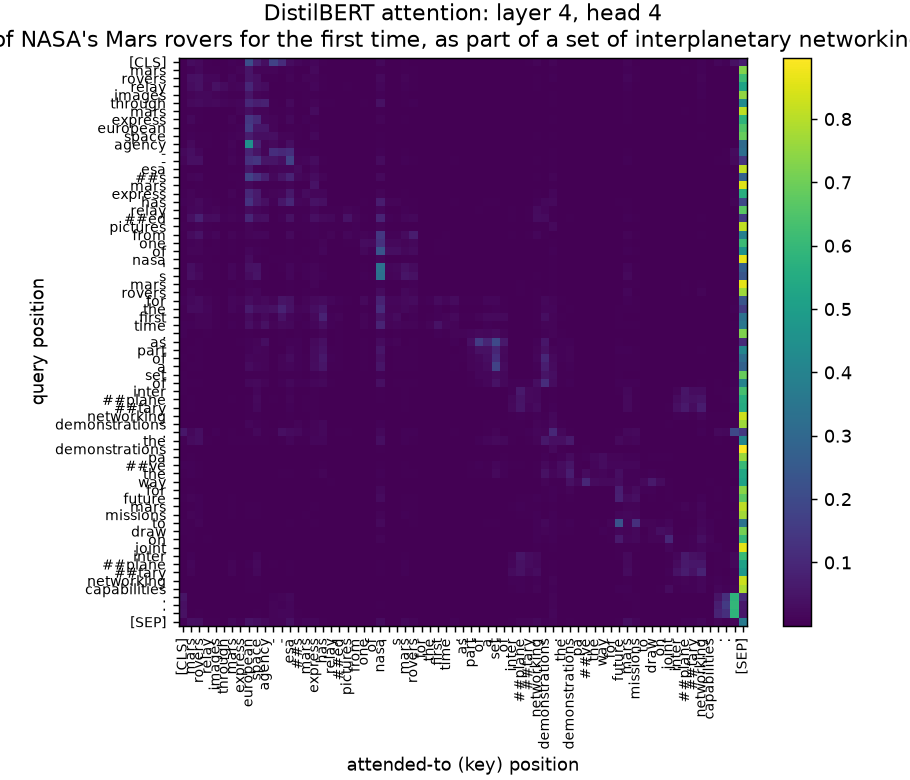
\includegraphics[width=0.85\textwidth]{figures/part_c_attention_heatmap.png}
    \caption{DistilBERT attention weights, layer 4 head 4.}
\end{figure}

The raw strongest link is \texttt{"demonstrations"} $\to$ \texttt{[SEP]} (weight 0.897) -- a
well-documented \textbf{attention-sink} pattern (heads dump weight onto \texttt{[SEP]} as a
low-information default). Restricted to content-word pairs, the strongest link is
\texttt{"agency"} $\to$ \texttt{"european"} (weight 0.449) -- a genuine \textbf{syntactic
compound-modifier} relation, within ``European Space Agency.''

\textbf{C4/C5 -- evaluation and comparison against Task 25's LSTM.} Identical test set (Task
25's \texttt{common.py} subsetting algorithm, byte-for-byte copied, verified to produce the
same examples).

\begin{table}[H]
\centering
\begin{tabular}{lrr}
\toprule
\textbf{Metric} & \textbf{DistilBERT} & \textbf{Best LSTM (GloVe+bidirectional)} \\
\midrule
Test accuracy & \textbf{0.9130} & 0.8840 \\
Macro F1 & \textbf{0.9130} & 0.8849 \\
Parameters & 66,956,548 & 2,236,548 (30x fewer) \\
Epochs to converge & \textbf{3} & 8 \\
\bottomrule
\end{tabular}
\end{table}

\begin{figure}[H]
    \centering
    
\includegraphics[width=0.55\textwidth]{figures/part_c_confusion_matrix.png}
    \caption{DistilBERT test confusion matrix.}
\end{figure}

\textbf{DistilBERT beats the LSTM by 2.9 accuracy points while converging in 3 epochs vs.\
8}, despite 30x more parameters. \emph{A note on wall-clock training time}: this run's
measured training time (4{,}201.6s) was significantly inflated by concurrent memory pressure
on the host machine (swap usage climbed to $\sim$5GB during training, confirmed via
\texttt{free -h}); freeing RAM measurably restored the expected per-epoch pace. This is
reported transparently rather than folded into the headline comparison, which would otherwise
overstate the Transformer's genuine wall-clock disadvantage versus the LSTM's 141.5s.

\textbf{C6 -- why performance/training characteristics differ (grounded in A/B).}
\textbf{(1) Pretraining, not architecture alone, drives the epoch-count gap}: DistilBERT
arrives already containing general English representations from large-scale pretraining --
fine-tuning only adapts them to 4 classes, unlike the LSTM's embeddings which had to learn
language structure from only 12,000 examples. \textbf{(2) Long-range dependency capture is
structurally easier}: every token pair interacts through one $O(1)$-path attention
computation (Part A1/A3), vs.\ the LSTM's cell-state highway which mitigates but does not
eliminate distance-dependent gradient attenuation (Task 25). This gap should widen further
for longer documents than AG News's short headlines. \textbf{(3) Sequence-length sensitivity}
runs the opposite direction at the extremes: Part B5's $O(n^2d)$ vs.\ $O(nd^2)$ analysis means
the Transformer's relative compute advantage shrinks (and eventually reverses) for $n\gg d$ --
a regime this short-sequence classification task does not stress-test.

% ----------------------------------------------------------------
\section*{Part D: Analysis \& Documentation}

\textbf{D1 -- pipeline summary.} Attention (Part A) replaces recurrence's sequential,
distance-decaying, fixed-bottleneck computation with $O(1)$-path, full-sequence-visible
weighted combination. Multi-head structure (B1) lets different relational patterns be
represented simultaneously rather than blended into one. Positional encoding (B2) is required
because attention is otherwise position-agnostic; sinusoidal PE specifically enables
closed-form relative-position representability and unbounded-length extrapolation. Encoder
(bidirectional context) / decoder (causally-masked, cross-attending to the encoder)
composition (B3) with residual+LayerNorm (B4, the same additive-shortcut fix as the LSTM's
cell-state highway, applied across layers instead of time) enables both stable deep-stack
training and the encoder-decoder division of labor.

\textbf{D2 -- quantitative findings, summarized.} See C4/C5/C6 above: DistilBERT +2.9
accuracy points over the best LSTM, 3 vs.\ 8 epochs to converge, at 30x the parameter count --
directly attributable to pretraining and attention's structural long-range-dependency
advantage, not merely "bigger model wins."

\textbf{D3 -- two non-trivial conceptual challenges.}

\emph{1. Extracting attention weights failed because of the attention \emph{implementation},
not the concept.} \texttt{output\_attentions=True} returned an empty tuple, easy to misread
as an indexing bug rather than what it was: the library's default fused \texttt{sdpa}
attention kernel never materializes the full $n\times n$ weight matrix, so there is nothing to
return. Resolved by loading with \texttt{attn\_implementation="eager"} -- a concrete
illustration of B5's efficiency-vs-transparency trade-off: a production optimization can trade
away exactly the intermediate quantity a conceptual analysis needs to inspect.

\emph{2. Understanding why sinusoidal PE needs \emph{paired} sin/cos, not sin alone.}
$\sin(pos\cdot\omega)$ alone doesn't determine $\cos(pos\cdot\omega)$, so there's no way to
recover the phase a linear map would need to compute $\sin((pos{+}k)\omega)$ from
$\sin(pos\cdot\omega)$ alone. Resolved by recognizing a $2$D rotation needs both coordinates
of a unit-circle point -- confirmed by implementing the explicit per-frequency rotation-matrix
construction and checking it reproduces true $PE(pos{+}k)$ to $\sim10^{-16}$ precision, rather
than trusting the trig identity alone.

\textbf{D4 -- reflection: limitations and a documented variant.} \textbf{Quadratic attention
cost} (B5): mitigated by sparse/local-attention variants (Longformer, referenced). \textbf{No
inherent order inductive bias} (B2): position must be externally supplied -- a genuine
trade-off (it's exactly what enables parallelism) rather than a pure downside, but a design
choice the architecture must get right. \textbf{A documented variant: Rotary Position
Embedding (RoPE; Su et al.\ 2021, used in LLaMA/GPT-NeoX)}, referenced without full
derivation -- rather than \emph{adding} a positional signal, RoPE rotates Q/K vectors by a
position-dependent angle so $Q_{pos}\cdot K_{pos'}$ becomes a function of relative offset
\emph{by construction}, not merely approximately recoverable via a learned linear map the way
sinusoidal PE only enables in principle -- empirically better length extrapolation than either
scheme this task derived. \textbf{Data/compute requirements}: Part C's whole applied
methodology (fine-tuning an already-pretrained model rather than training from scratch) \emph{is}
the standard, practical response to this limitation, not a convenience specific to this task.

\end{document}
